\section{SMELLIE Beam Profiling}\label{sect:beam_profiling}
% TODO:
% - First section: description of how SMELLIE events have previously been simulated. Things to simulate correctly: position, initial direction, intensity, wavelength distribution, and of course angular emission profile (the beam profile).
% - For the latter, give detail about why 1D approach didn't seem to work, and why Esther chose 2D method. Outline her 2D generator method, as well as issues with it: slow! Only one run used per fibre.
% - Explain new generator approach: using an inverse-CDF approach, 2D histogram binned in angles (phi, r=1-cos theta). Describe algorithm.
% - Explain statistical approach for multiple data sets were combined together: maximum-likelihood approach. Note the assumptions made for this statistical model of our data (wavelength independence, Poisson data, etc.)
% - Demonstrate results, validation - is it faster, of better quality than before? How does one define quality here?
\subsection{Previous attempts at SMELLIE event simulation}
Critical to extraction of scattering information from SMELLIE data is an accurate Monte Carlo (MC) simulation of the SMELLIE system. By modelling the laser light emission into the detector correctly, we can simulate how SMELLIE light will be impacted by changing scattering lengths in the detector. Because of the complexity of the optics of the optical fibres used to direct the laser light into the detector, a given SMELLIE event is simulated as a point-like ``flash" of visible photons emanating from the emission point of the fibre into the detector. This flash then requires a number of parameters to be correctly described. In particular, the fibre emission positions were recorded during the installation of the fibres. The wavelength and timing distributions were taken from measurements of the laser heads by their manufacturers, or by colleague Jeff Lidgard in the case of the SuperK wavelength distribution. The intensity is defined as the mean number of photons simulated per event; on an event-by-event basis we sample Poisson fluctuations about that mean intensity value. Determination of intensity must be done on a subrun-by-subrun basis. Unlike scintillation light, light from SMELLIE is not at all isotropic, and so we must specify some form of angular emission distribution. Determining and handling these angular emission distributions, also known as beam profiles, is the focus of this chapter.

Before we can determine the beam profiles, we must first decide how to specify them. Previous observations show that different fibres can have notably different angular profiles~\cite{majumdar_measurement_2015}, so we let each fibre's beam profiles be unique. We assume for now that a given fibre's beam profile is stable over time, and independent of the wavelength of light fired. A straightforward, na\"{i}ve approach to parameterising a beam profile would be as follows: specify some nominal fibre direction, corresponding to the direction light takes travelling from the fibre to the centre of the ``beamspot'' on the other side of the detector. Then, specify a 1D angular distribution, corresponding to the probability density of firing a photon at a given polar angle $\alpha$ relative to the nominal direction. One might even assume this distribution is Gaussian in shape. The distribution in azimuthal direction, $\phi$, is assumed to be uniform.

\begin{figure}
    \centering
    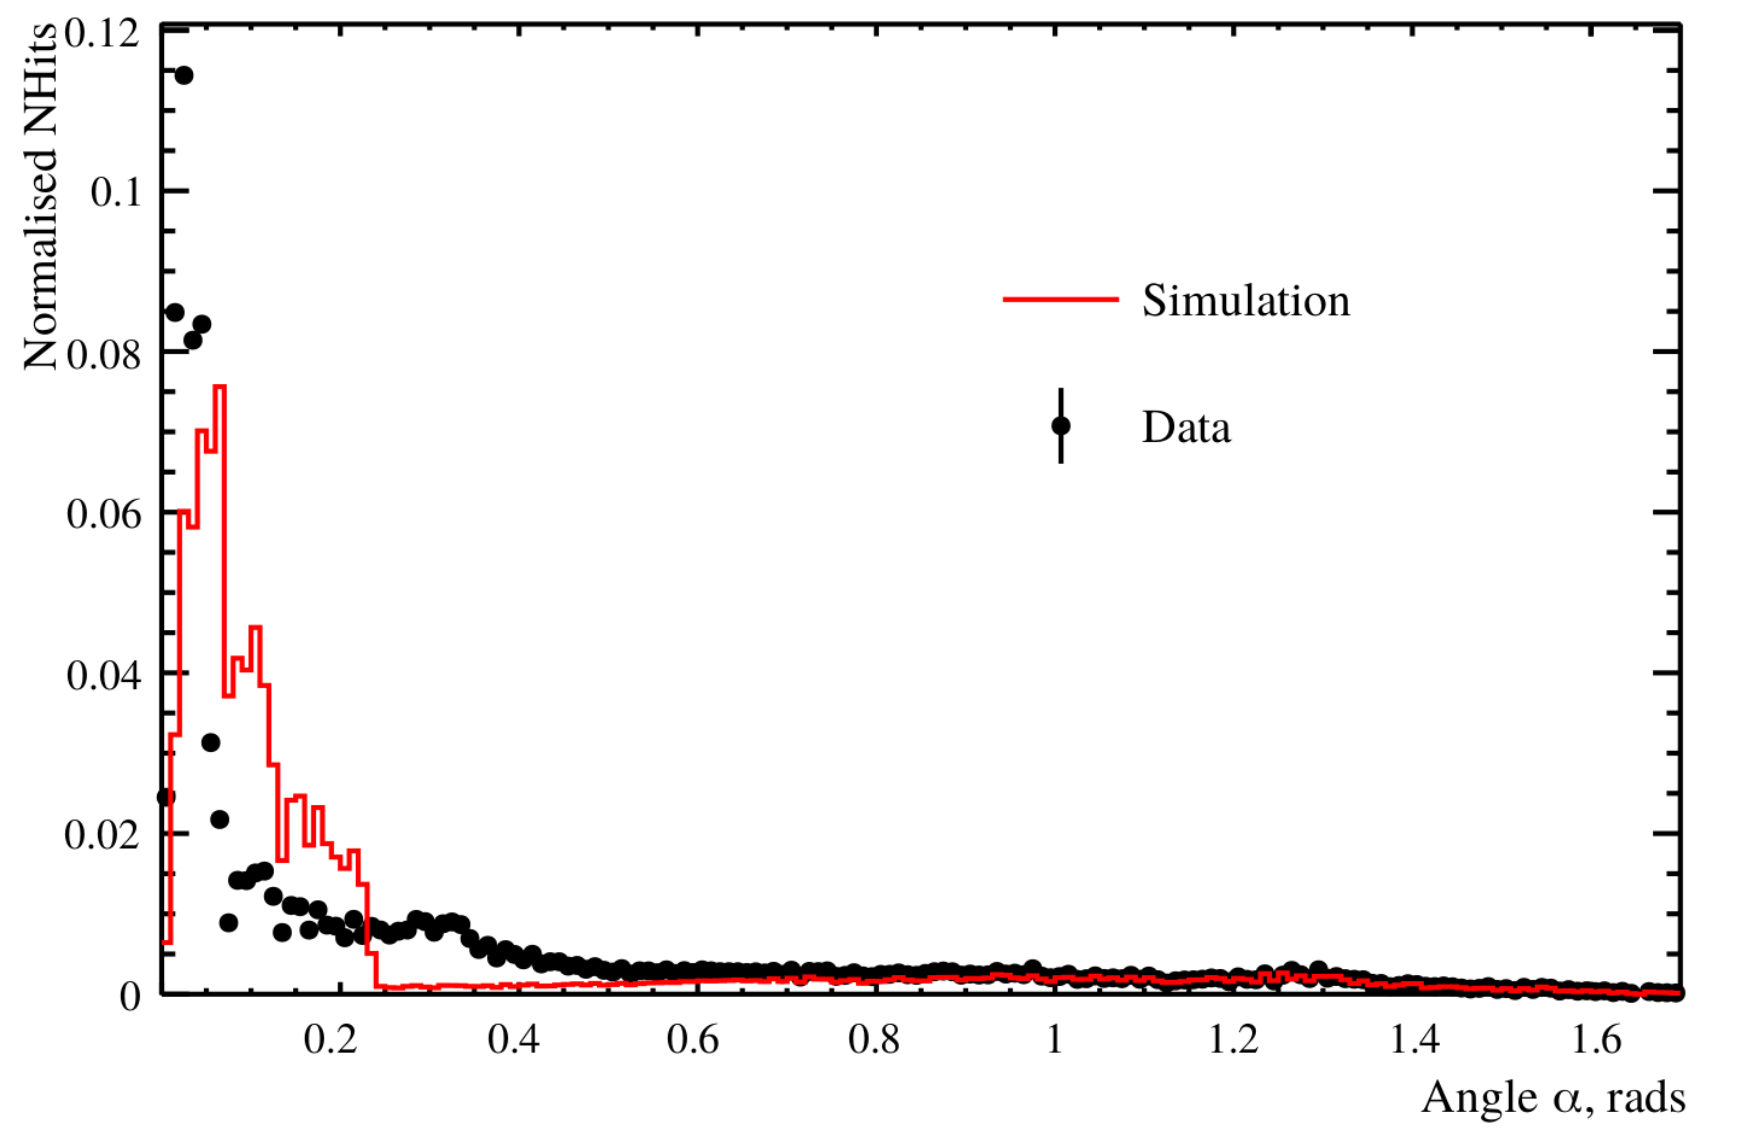
\includegraphics[width=0.7\textwidth]{images/1D_gen_plot.png}
    \caption{Comparison between a simulation of one of the fibres, made from the 1D beam profile generator (red), with the associated data subrun that was used to create that beam profile (in black). For both MC and data, what is plotted is the PDF of observed PMT hits, as a function of the $\alpha$ angle. Poisson errors on the data points have been added, but are too small to see. Clearly, this 1D generator does not replicate the observed angular distribution correctly. Figure taken from~\cite{turner_measurement_nodate}.}
    \label{fig:1d_gen_plot}
\end{figure}

This 1D beam profile approach is currently used by both TELLIE and AMELLIE for their simulations, and was used initially for SMELLIE. However, when SMELLIE data was taken in the water-phase of the experiment, simulations using these beam profiles failed to match them well at all - see figure~\ref{fig:1d_gen_plot} for an example. Not only was the distribution in $\alpha$ not Gaussian, a distinct speckle-pattern can be observed within the beamspot that is not uniform in $\phi$. This fact led to colleague Esther Turner building a SMELLIE generator that could handle 2D beam profiles: angular emission distributions dependent on both $\alpha$ and $\phi$. The distribution was stored as a mapping from each inward-pointing PMT in the detector to a relative intensity value. This was chosen because the beam profile shapes were calibrated from existing SMELLIE data --- more on this in section~\ref{sect:new_beam_profiles}.

This original 2D generator then sampled the beam profile via a rejection sampling approach, outlined as follows:
\begin{enumerate}
    \item Propose a test direction $(\alpha, \phi)$, by generating $\phi$ uniformly in the interval $[0, 2\pi]$, and $\alpha$ according to some pre-determined Gaussian distribution, known as the Gaussian envelope.
    \item Given this test direction, calculate where a line following this direction from the fibre of interest will hit the PSUP on the other side of the detector. Find the 3 closest PMTs to that point.
    \item From those PMTs, obtain their relative intensity values from the beam profile mapping, and perform an interpolation based on how close each PMT is to the PSUP intersection point. This gives an interpolated relative intensity value for this test direction.
    \item Because we are sampling using the angular coordinates $(\alpha, \phi)$, differential area elements over this space of directions do not have the same size. We can correct for this fact by multiplying our interpolated relative intensity by $\sin{\alpha}$, which corresponds to the Jacobian of the direction-space.
    \item Calculate the value for the Gaussian envelope along this test direction.
    \item Throw a random number uniformly between 0 and the Gaussian envelope value. If the random number is less than the interpolated intensity, then this test direction is accepted, and a photon is generated with that direction. Otherwise, we reject the direction and try the whole process again.
\end{enumerate}

This generator certainly works, but has a key problem: efficiency. The 1D generator was able to generate a SMELLIE event (that is, to fully specify the starting parameters of all the photons emitted from a fibre) at a speed of $\sim\SI{1}{\milli\second}$. However, the 2D generator specified here could take upwards of $\sim\SI{50}{\second}$ \textit{per event} to generate. Because a typical SMELLIE analysis requires simulating many millions of events, the CPU time taken to perform this quickly became unfeasible. Fixing this generator speed problem was a high priority for the SMELLIE analysis.

\subsection{The new generator}\label{sect:new_gen}
On careful inspection of the existing 2D generator, the main reason for the slowness of the algorithm is the use of a rejection approach. Even with use of the Gaussian envelope, which was included to help with speed, the vast majority of proposed directions are never selected. Figure~\ref{fig:num_attempts} shows a histogram of number of attempts per event it took for a valid direction to be chosen for a representative SMELLIE simulation. Moreover, the calculations needing to be done for every proposed direction are relatively complex, notably trying to find the 3 nearest PMTs to some point on the PSUP.

\begin{figure}[ht]
    \centering
    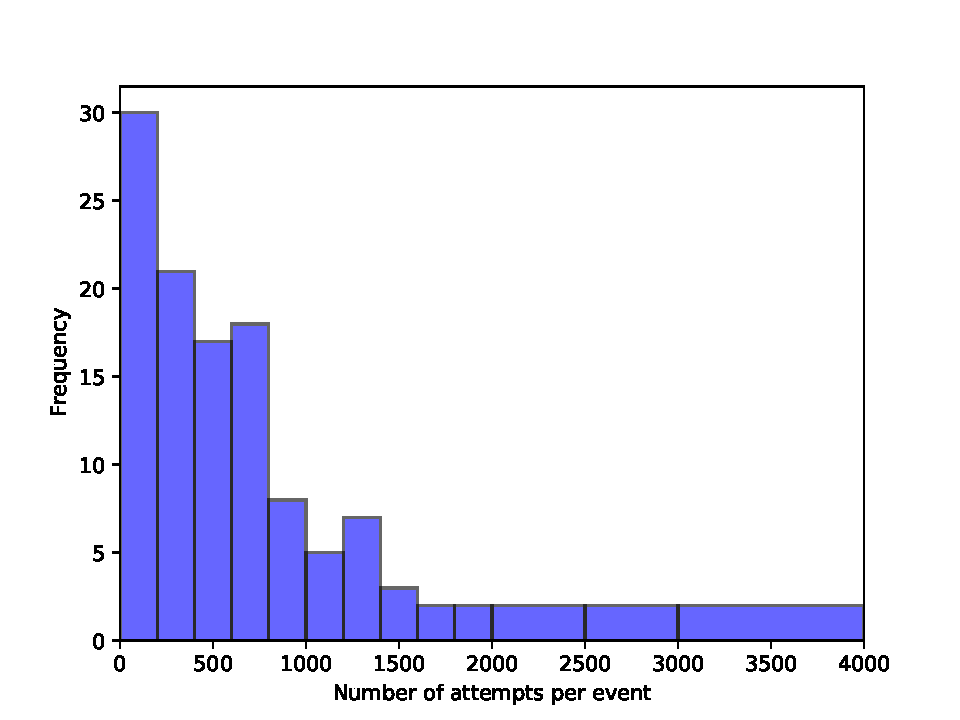
\includegraphics[width=0.7\textwidth]{images/2D_generator_num_attempts_nicer.pdf}
    \caption{Typical distribution of the number of attempts it takes for the existing 2D generator before the test direction gets accepted, per event.}
    \label{fig:num_attempts}
\end{figure}

A new 2D generator was built with these thoughts in mind. Firstly, the rejection method would no longer be used, given its inefficiency. We would also endeavour to try and ``pre-calculate'' as much as possible before run-time. Starting with the existing PMT relative intensity maps, we plot these in the 2D direction-space $(1-\cos\alpha, \phi)$: see Figure~\ref{fig:esther_beam_profile}. In a toy-MC simulation, \num{500000} directions are then thrown uniformly in this 2D space per fibre. For each direction, the same method of obtaining an interpolated intensity value from the nearest PMTs to the corresponding point on the PSUP as from the original 2D generator was performed, the only difference being that these calculations were done well before any actual SMELLIE simulation. Figure~\ref{fig:old_profile_interpolated_sample_plot} shows the interpolated intensities obtained for one fibre.

\begin{figure}[ht]
    \centering
    \begin{subfigure}{0.48\textwidth}
        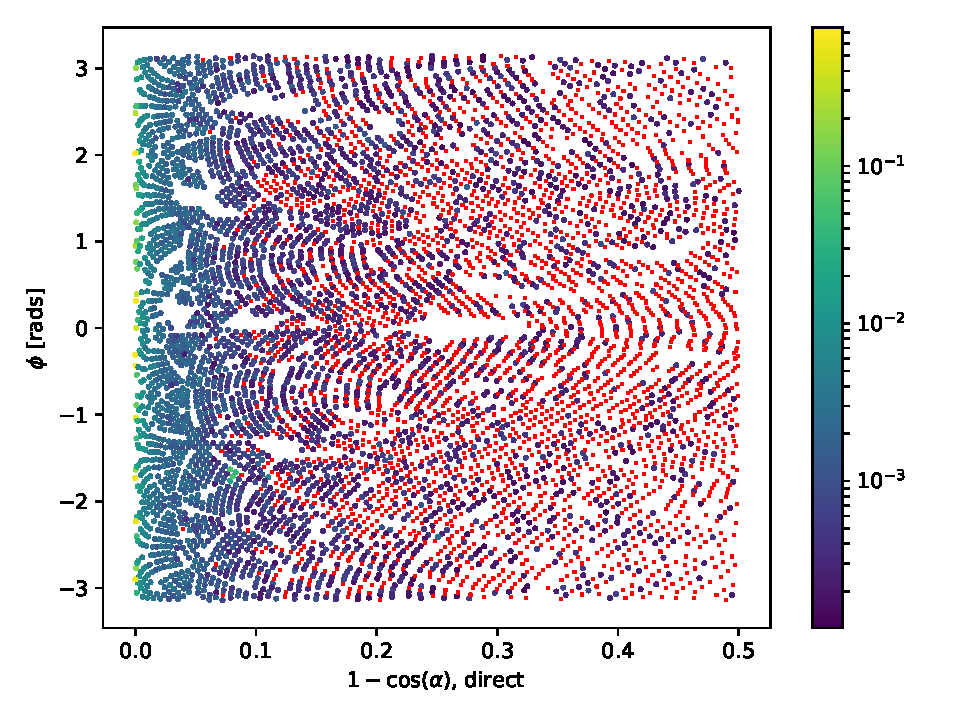
\includegraphics[width=\textwidth]{images/flat_plot_r_FS055_beam_profile_original_6-18-13.pdf}
        \caption{PMT relative intensity map}
        \label{fig:esther_beam_profile}
    \end{subfigure}
    \begin{subfigure}{0.48\textwidth}
        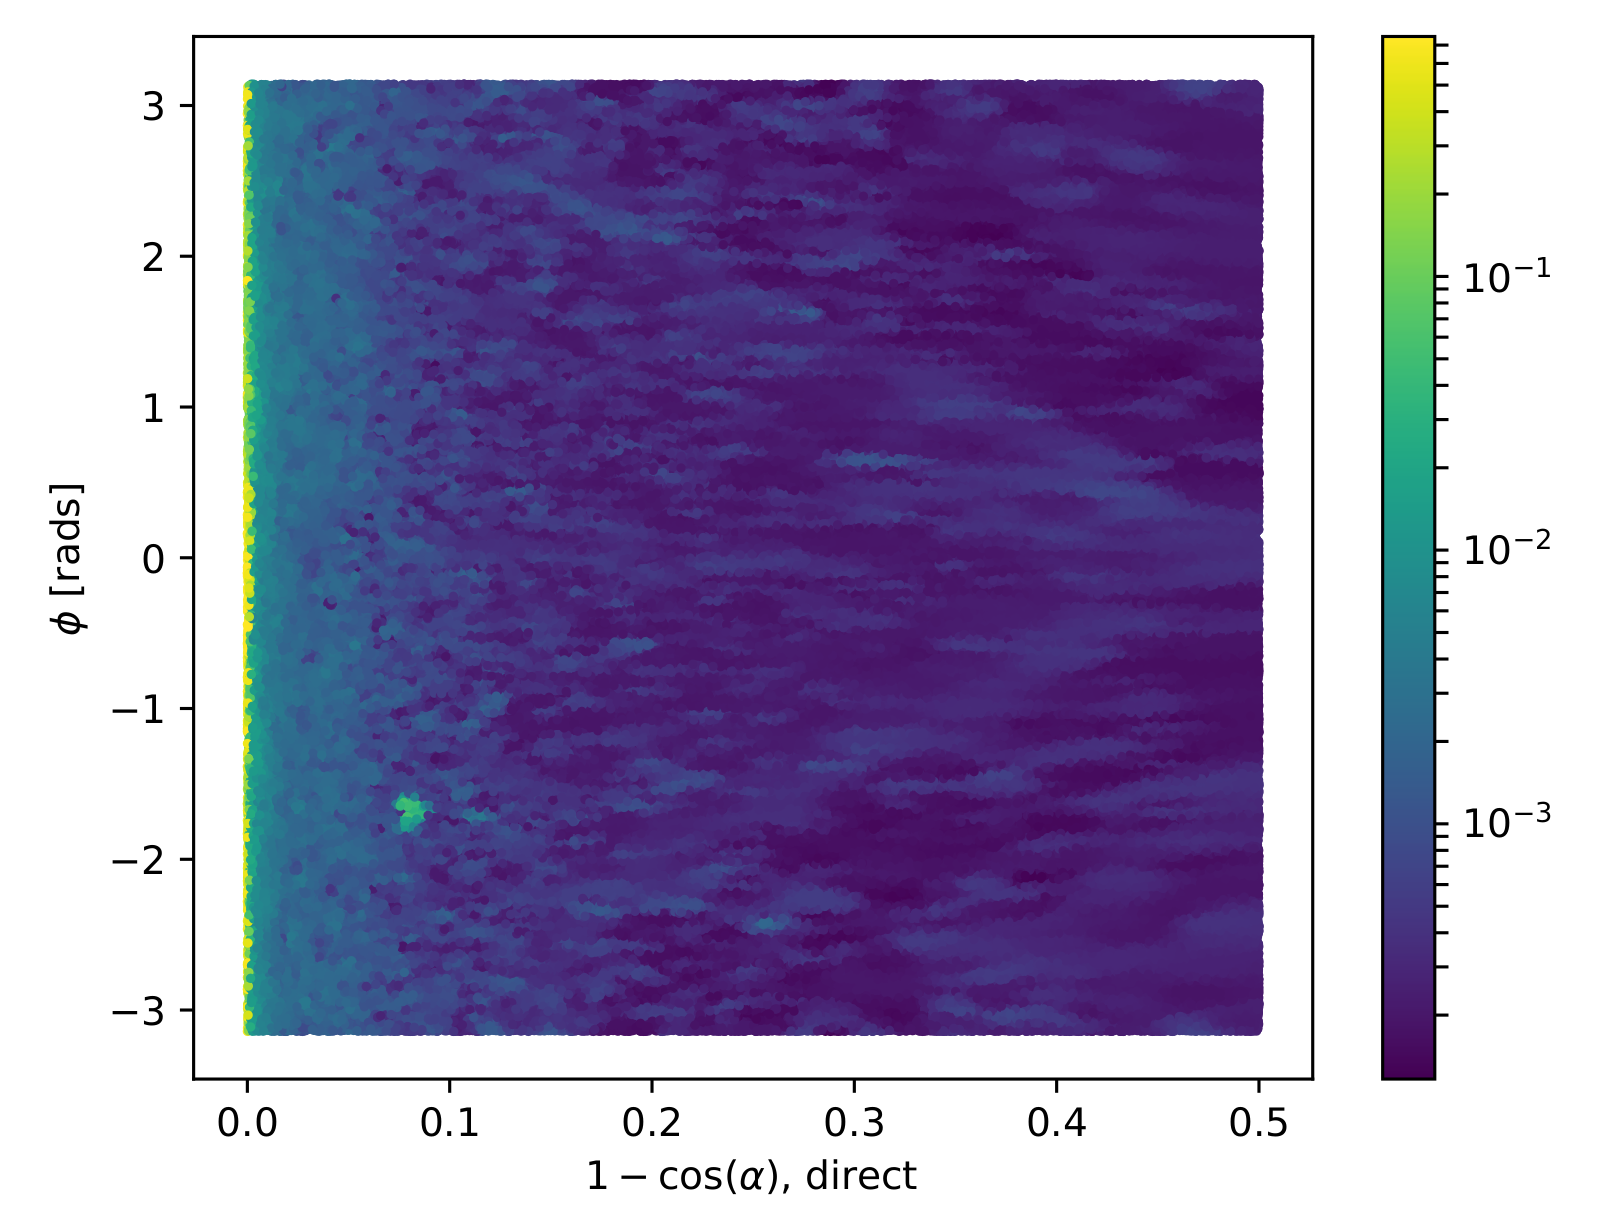
\includegraphics[width=\textwidth]{images/polar_plot_FS055_MC_sampling_old_beam_profile.png}
        \caption{Interpolated intensity map}
        \label{fig:old_profile_interpolated_sample_plot}
    \end{subfigure}
    \caption{The first step in the new method for preparing the new generator. In (a), the relative intensities used for the existing beam profile of fibre labelled FS055 are shown for each PMT, the position on the plot indicating the location of that PMT in the fibre coordinates. The colour indicates the relative intensity; PMTs marked red have an intensity of zero. Figure (b) shows the result of throwing \num{500000} directions uniformly over this 2D space, the intensity of each point given by interpolating the intensities of nearby PMTs.}
    \label{fig:esther_beam_profile_and_interp}
\end{figure}

Following this, the sampled intensities were then binned into a 2D histogram, where the bin value corresponds to the sum of all intensities for all directions found within this bin. Choosing a sensible binning procedure is important: too few bins, and necessary information about the shape of the beam is lost, whilst too many bins can oversample the data and capture statistical artefacts in the sampling process instead of just the beam profile. As a balance, 15 bins were chosen along the $\phi$ direction, and 60 in $r=1-\cos\alpha$. This was chosen to ensure that a reasonable number of PMTs were located within each bin, lessening the impact of any statistical fluctuations. Although the bins in $\phi$ were chosen to have uniform width, this was decided to be not the case for the other axis, as there is far more important information near $r = 0$ (the beamspot). Instead, the width of the bins in $r$ were calculated so that roughly the same total probability was contained in each $r$-strip. By consequence, bins near the beamspot typically are of significantly smaller size than ones much further out. This allows us to both capture any rapid changes in intensity near the beamspot, where this matters greatly, as well as smooth out the very-low intensities seen at larger polar angles. One of these histograms can be seen in Figure~\ref{fig:hist_cdf_old_profile}: the large change in bin widths as a function of $r$ is clear. One can also see that near the beamspot notable dependence on the intensity as a function of $\phi$. The mysterious ``spot'' at $r = 0.08$, well out of the beamspot, is an indication that the underlying beam profile data being used requires improvement: more on this in section~\ref{sect:new_beam_profiles}.

\begin{figure}
    \centering
    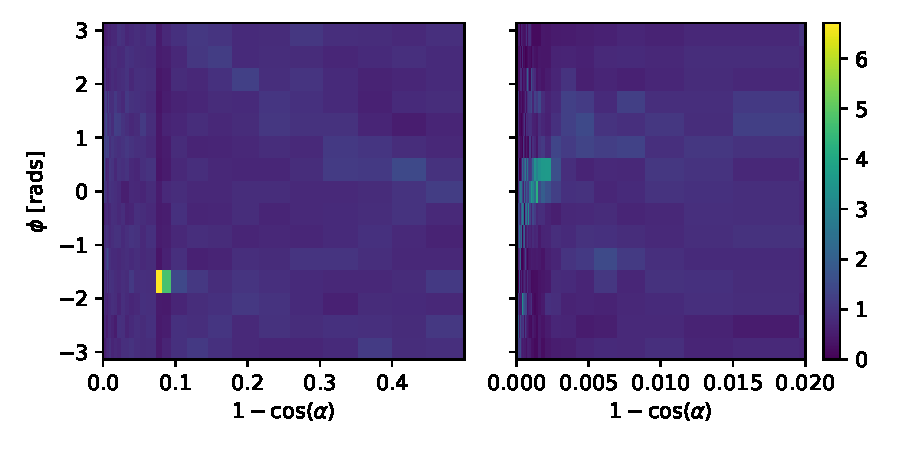
\includegraphics[width=\linewidth]{images/FS055_60_alpha_15_phi_hist.pdf}
    \caption{Histogram of interpolated intensities within the 2D direction-space. The left view shows the full histogram; the right is a zoomed-in version near the beamspot. Unlike the binning in $\phi$, the bin widths in $r$ are not at all uniform. Instead, they have been determined such that the area summed over a given ``strip" of bins of constant $r$ will be the same.}
    \label{fig:hist_cdf_old_profile}
\end{figure}

The Cumulative Density Function (CDF) of this intensity histogram as a function of bin was then produced, where the bins were ordered through a raster-scan: scanning first over $\phi$, and then $r$. The CDF was then normalised to 1 so that it was well-defined. It is this CDF object that is then loaded in and sampled from during event generation. To do this, an ``inverse-CDF'' approach was used, which has the major benefit over rejection sampling of always producing a valid direction for every sample made. The algorithm works as follows:

\begin{enumerate}
    \item Throw a random number uniformly in $[0,1]$.
    \item Perform a binary search to find the bin that has the largest CDF value below this random number.
    \item Look at the bin edges in $\phi$ of this selected bin: use linear interpolation of the random number to obtain a $\phi$ value located between these two $\phi$-values.
    \item Look at the the selected bin's $r$-bin edges, and select a value of $r$ by throwing a second random number uniformly between the two edges. Convert this $r$ into a polar angle $\alpha$.
    \item The photon's direction is defined by the $(\alpha, \phi)$ chosen by this process. 
\end{enumerate}

Because of the relative simplicity of this algorithm compared to the previous 2D generator, the speed improvement was very large: generation now took $\sim\SI{1}{\milli\second}$ per SMELLIE event, a speed improvement of nearly $\num{50000}$. Event generation became as fast as it was when the 1D generator was being used. Furthermore, because of the approach taken, this major speed improvement comes at no sacrifice in accuracy. Figure~\ref{fig:data_generator_comp_new_profiles} shows a comparison of the average number of photoelectrons (npe) per event per PMT between water-phase SMELLIE data and simulations with both the old and new 2D generator. One can see clearly that both generators are as accurate as one another. Note that this plot uses the updated beam profiles as explained in the next section.

\begin{figure}
    \centering
    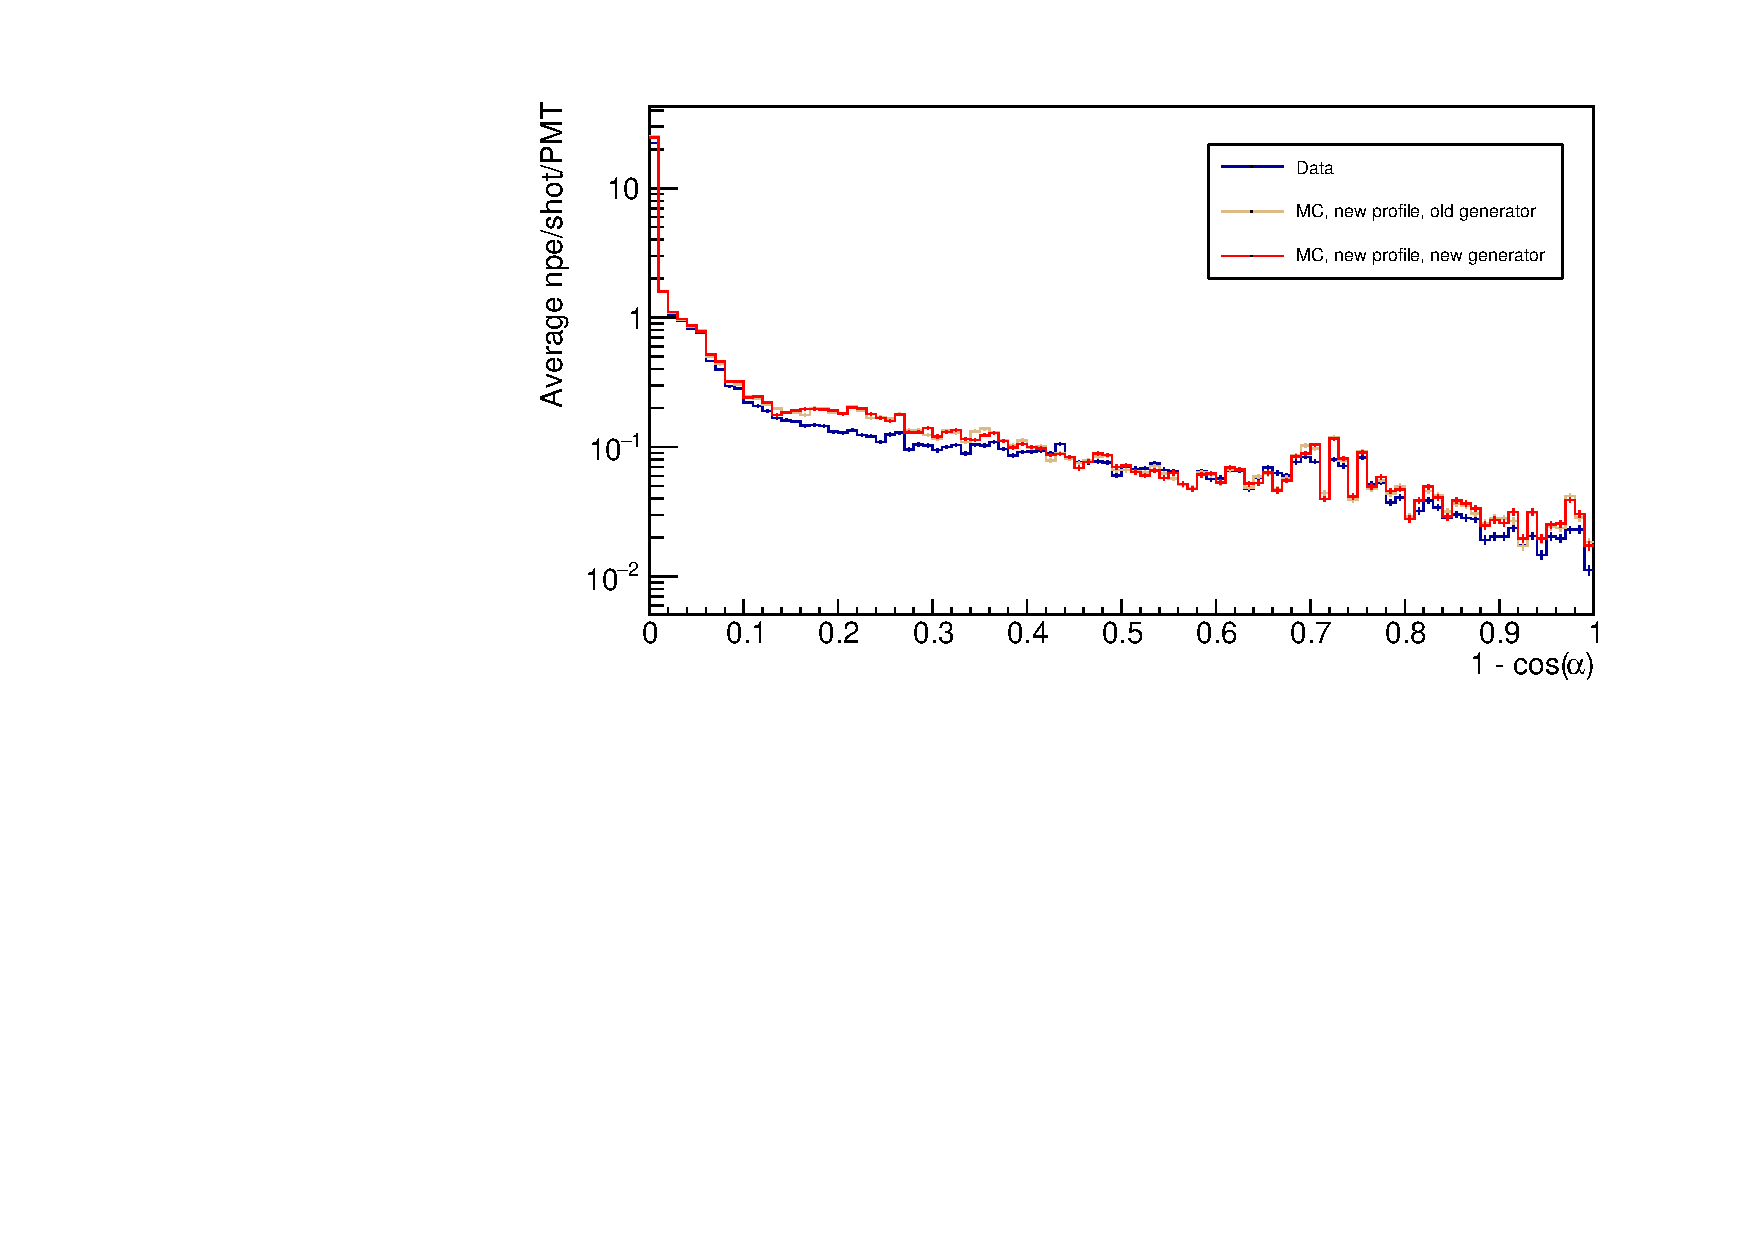
\includegraphics[width=\linewidth]{images/data_vs_MC_new_profiles_new_and_old_generators_npe_r.pdf}
    \caption{Comparison of water-phase data to MC generated using both the old and new 2D beam profile generator approaches, with the updated beam profiles. Both versions of the generator are consistent with one another, but the new generator is many time faster.}
    \label{fig:data_generator_comp_new_profiles}
\end{figure}

\subsection{Improving the beam profiles}\label{sect:new_beam_profiles}
Even with the new 2D profile generator, a problem remains: the simulation fails to reasonably recreate data, and much of this appears to be because of the poor beam profile data being used. The curious ``spot'' for one of the fibres was already noted in the previous section that doesn't seem to be physical, and more broadly at large angles for all the fibres there are large swathes of PMTs with an intensity of zero, providing little useful information about the beam shape. It was shown in~\cite{turner_measurement_nodate} that with the old 2D generator, the systematic uncertainty on the beam profiles was the dominant source of error in the main SMELLIE analysis. To help improve this situation, it was decided to update the existing beam profiles.

These old beam profiles were originally determined by looking at SMELLIE data taken during the water-phase. Specifically, a ``medium''-intensity subrun with one of the lasers firing at a long wavelength, \SI{495}{\nano\metre}, was chosen for each fibre. ``Medium''-intensity corresponds to firing the relevant laser at a set intensity determined during an earlier commissioning process, for which the maximum occupancy of PMT hits at that intensity, i.e. the proportion of hits per event, corresponded to roughly 80\%. This value was chosen as it allowed for high statistics in a relatively short run-time, but not so intense that the occupancy of any given PMT in the beamspot was 100\%. Because Rayleigh scattering is strongly-dependent on wavelength, the long wavelength of light was chosen so that impacts from this scattering were small in the data.

SNO+ PMTs are unable to distinguish between one or more photoelectrons being generated (except for very large numbers, at which point the charge collected can provide some useful discriminating power). As a result, the occupancy of a PMT over a number of SMELLIE events, $o$ is a biased estimator of the mean number of photoelectrons generated, $\mu$. Assuming the number of photoelectrons generated in a given event follows Poisson statistics, the probability of generating k photoelectrons is:

\begin{equation}
    P\left(k | \mu\right) = \frac{\mu^{k}e^{-\mu}}{k!}.
\end{equation}

The probability of observing a ``hit'' in a given PMT corresponds to generating at least one photoelectron:

\begin{equation}\label{eq:p_hit}
    P\left(\text{hit}| \mu\right) = P\left(k\geq 1 | \mu\right) = 1 - P\left(k = 0 | \mu\right) = 1 - e^{-\mu},
\end{equation}
which implies after rearrangement that one can determine the mean number of photoelectrons per event from the occupancy by:
\begin{equation}\label{eq:multihit_correction}
    \mu = \ln\left(1 - o\right).
\end{equation}
This is the reason why we want to avoid PMTs with occupancies of 100\%: they preclude one's ability to convert into a value for $\mu$ by looking at occupancy alone. We call this conversion from occupancy into npe the ``multi-hit correction''. The impact of this correction is typically small for most PMTs, but can become very significant in a fibre's beamspot.

Once the npe mapping from data was obtained, a correction was then made for the detector's optics: even ignoring a fibre's angular distribution, we still expect certain PMTs to be illuminated more than others because of e.g. reflections off of the AV, or the solid angle subtended by the PMT bucket opening. For each fibre, a simulation was made where the beam profile was set as uniform, and the corresponding npe mapping obtained: this map held information about the detector optics only. The beam profile mapping was then derived by simply dividing each fibre's npe mapping from data to its associated isotropic MC npe map. It is these maps that were first used in section~\ref{sect:new_gen}.

\subsection{Combining beam profile datasets}
Fortunately, much more SMELLIE data was taken during the water-phase than was used for the original beam-profiling analysis. This additional data can be combined with that which was already used to far better constrain the beam profiles. In particular, given the existing assumption that scattering effects are minimal above wavelengths of $\sim\SI{490}{\nano\metre}$, all data taken with wavelengths above this can also be used. The specific runs (and associated comments about their specifics) are described in Table~\ref{tab:runs_used}. Because high-intensity runs require a different analysis approach (PMTs with high occupancies must use charge, not occupancy, to  estimate npe), for this analysis we only considered subruns that used low or medium intensity set-points.
\begin{center}
    \begin{table}
        \begin{tabular}{c p{6cm} p{6cm}}
            \hline
            Run Number & Run Type & Comments \\ \hline \hline
            \num{114018} & All PQ lasers; SuperK laser in \SIrange{400}{500}{\nano\metre} range & Only PQ495 laser and SuperK at \SI{495}{\nano\metre} is used \\
            \num{114023} & SuperK laser in \SIrange{500}{600}{\nano\metre} range & Part 1 of this wavelength range; crash occurred on last subrun, so that subrun is ignored \\
            \num{114034} & SuperK laser in \SIrange{500}{600}{\nano\metre} range & Part 2 of this wavelength range \\
            \hline
        \end{tabular}
        \caption{Water-phase runs used for new beam profiling.}
        \label{tab:runs_used}
    \end{table}
\end{center}
For each subrun $j$ of data per fibre, we look only at PMT hits for each PMT $i$ that has been identified as ``good'' for that subrun, $i \in G_{j}$\footnote{Strictly speaking, a PMT's ``goodness'' is only determined on a run-by-run, not a subrun-by-subrun level, but this has no impact on the analysis.}. In particular, a ``good'' PMT must have valid electronic and timing calibrations, be at high voltage and masked into the detector's trigger system for that subrun. In addition, an angular cut of $\alpha < \SI{60}{\degree}$ was made to remove PMTs that are well outside of any reasonable beam direction. To isolates the hits arriving directly from the fibre without reflecting, scattering, or being noise, a time cut was also made. Because what matters is the time relative to emission from the fibre, and the expected time-of-flight from fibre to different PMTs varies, a quantity known as the time residual was used. Starting with the calibrated hit time of a given PMT $t_{hit}$, the expected time-of-flight $t_{TOF}$ was subtracted off, estimated with the collaboration's ``Light Path Calculator''. Then, the emission time was also subtracted off, $t_{emm}$, estimated by looking at the second-earliest value of $t_{hit}-t_{TOF}$ within the fibre's beamspot, defined as the PMTs for which $\alpha<\ang{3}$. It was found that a ``loose'' time residual cut of $t_{res} \in [-10, +12] \si[]{\nano\second}$ was sufficient to remove the vast majority of non-direct light with little signal sacrifice. In the situation where a subrun with intensity was very small, it would not regularly have at least two hits in the beamspot, and so the time residuals calculated would not be valid for many events. To avoid this situation, a cut was made on any subruns with mean intensities below 9. This value was chosen as it would mean a fluctuation downwards of $2\sigma=2\cdot\sqrt{9}=2\cdot3=\SI{6}{\npe}$ would still have more than the 2 hits necessary for timing reconstruction.

Extracting the underlying beam profiles from these data required some careful thought, especially because subruns could have wildly-varying intensities. Considering a PMT $i$ in subrun $j$, the mean number of photoelectrons generated per event in that PMT for that subrun, $\mu_{ij}$ can be decomposed as follows:

\begin{equation}\label{eq:mu_def}
    \mu_{ij} = I_{j}k_{i} = I_{j}b_{i}f_{i}.
\end{equation}
$I_{j}$ is the intensity of the subrun, i.e. the mean number of photons generated from the fibre in that subrun per event. $k_{i}$ is the probability that a given photon generated at the fibre source ends up generating a photoelectron in PMT $i$. This itself can be further split into two components: $b_{i}$, the probability that a given photon at the fibre source points in the direction of PMT $i$; and $f_{i}$, the probability that a given correctly-pointed photon actually makes it to the PMT and successfully generates a photoelectron. It is $b_{i}$ that is the actual beam profile we would like to measure.

Letting $p_{ij}$ be the probability of observing a hit for a given event on a given PMT, the probability of observing $m_{ij}$ hits out of $N_{j}$ events in the subrun will be binomially-distributed:
\begin{equation}
    P(m_{ij} = m | \mu_{ij}) = L(\mu_{ij} | m_{ij} = m) = \binom{N_{j}}{m}p_{ij}^{m}(1-p_{ij})^{N_{j}-m} = \binom{N_{j}}{m}\left(1-e^{-\mu_{ij}}\right)^{m}e^{-\mu_{ij}(N_{j}-m)}.
\end{equation}
Here we have used equation~\ref{eq:p_hit}, and noted that this probability distribution in $m$ can be re-framed as a likelihood function for the parameter $\mu_{ij}$. Considering only a single subrun of data, the maximum likelihood estimate of the parameter $\mu_{ij}$ can be shown to be:
\begin{equation}
    \left<\mu_{ij}\right> = -\ln\left(1-\frac{m_{ij}}{N_{j}}\right) = \ln\left(1-o_{ij}\right) \qquad(m_{ij} \neq N_{j}),
\end{equation}
where $o_{ij}$ is just the occupancy of PMT $i$ in subrun $j$. This is just the multi-hit correction formula seen in equation~\ref{eq:multihit_correction}, which makes sense.

When looking at multiple subruns for the same fibre, the total likelihood function for a given PMT when considering all of the data for a given fibre will be the product of the likelihoods from each dataset,
\begin{equation}
    L\left(\left\{I_{j}\right\}, k_{i} | \left\{m_{ij}\right\}\right) = \prod_{j} L(I_{j}, k_{i} | m_{ij}) = \prod_{j}\binom{N_{j}}{m_{ij}}\left(1-e^{-I_{j}k_{i}}\right)^{m}e^{-I_{j}k_{i}(N_{j}-m)}.
\end{equation}
This leads to a log-likelihood distribution of
\begin{equation}
    \mathcal{L}\left(\left\{I_{j}\right\}, k_{i} | \left\{m_{ij}\right\}\right) = \sum_{j}\left[\ln\left(^{N_{j}}C_{m_{ij}}\right) + m_{ij}\ln\left(1 - e^{-I_{j}k_{i}}\right) - I_{j}k_{i}\left(N_{j} - m_{ij}\right)\right].
\end{equation}
Formally, one could combine the likelihoods of all the PMTs together, and by looking at the maximum likelihood estimates for each of the parameters measure the parameter values this way. However, the set of equations one obtains through this approach quickly become analytically intractable, because the PMTs are coupled by the intensity values $I_{j}$. Even a direct numerical approach would be liable to fail: for a given fibre there can be dozens of subruns, and many thousands of PMTs of relevance, so the dimensionality of the system of equations would be far too large.

Because of this, a different approach was taken. It is expected that in a subrun the total npe, summed over all good PMTs, should be proportional to the intensity value $I_{j}$. One must be careful about this construction --- different subruns can have different sets of good PMTs, so two subruns with identical $I_{j}$ values could have a larger summed npe merely because more PMTs were good in that subrun. To counter-act this effect, only PMTs that were classified as good in \textit{all} subruns being analysed for that fibre would be used for the npe summation. In other words, we use data from PMT $i$ for summing only if:
\begin{equation}
    i \in I = \bigcap_{j}G_{j}.
\end{equation}
By finding a value proportional to $I_{j}$, there is now enough information to maximise the log-likelihood $\mathcal{L}\left(k_{i} | \left\{m_{ij}\right\}, \left\{I_{j}\right\}\right)$ with respect to $k_{i}$ for each PMT independently, and hence obtain estimates for these $k_{i}$ parameters.

Of course, what is actually wanted are the underlying $b_{i}$ values, not $k_{i}$. This is where isotropic simulations come in. For each run of data used, a matching isotropic MC was produced. For example, a simulation for run \num{114023} contained \num{10000} events for each fibre using an isotropic beam profile, over the full wavelength range considered in this run, \SIrange{500}{600}{\nano\metre}, using the same run conditions as in data (which PMTs were live, etc.).

For each isotropic MC run, both $I_{j}^{MC}$ and $k_{i}^{MC}$ were calculated via the method described above. Because the simulations were isotropic, the underlying value for $b_{i}$ was constant across all the PMTs, and so $ak_{i}^{MC} = f_{i}$. By doing some rearranging of equation~\ref{eq:mu_def}, we find that:
\begin{equation}
    \mu_{ij} = I_{j}b_{i}f_{i} = cS_{j}b_{i}ak_{i}^{MC} = (acb_{i})S_{j}k_{i}^{MC}.
\end{equation}
As a result of this, given the set $\left\{S_{j}\right\}$ and $k_{i}^{MC}$, one can maximise the log-likelihood $\mathcal{L}$ with respect to $b'_{i} = acb_{i}$ numerically, to obtain the maximum likelihood estimate of $b'_{i}$. Because $a$ and $c$ were global constants of proportionality, they would become irrelevant as soon as the beam profile was normalised in the CDF-creation process outlined in~\ref{sect:new_gen}.

Figure~\ref{fig:likelihood_scan} shows the shape of this log-likelihood distribution for a particular PMT when considering fibre FS007's beam profile. One can see how individual subruns provide much more information when combined together, than if one looked at a single subrun alone.

\begin{figure}
    \centering
    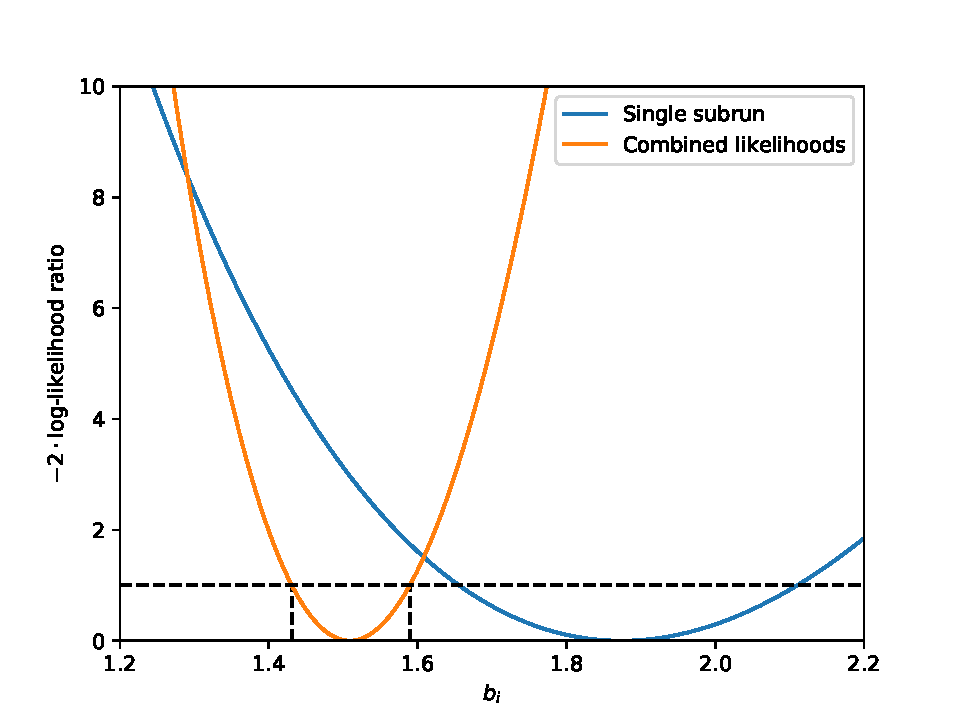
\includegraphics[width=\linewidth]{images/example_likelihood_distribution_pmt.pdf}
    \caption{Plot of $X_{i}$, equal to twice the negative log-likelihood ratio, for both a single subrun of a typical PMT, and when all relevant subruns are combined together. Also shown with the dotted lines is the production of a $1\sigma$ confidence interval, by seeing where the value of $X_{i}$ equals 1.}
    \label{fig:likelihood_scan}
\end{figure}

Another benefit of using this log-likelihood approach is that the resulting distribution's shape can be used for uncertainty estimation. In almost all cases, Wilks Theorem~\cite{wilks_large-sample_1938} allows us to produce $1 \sigma$ confidence intervals about the maximum likelihood estimate for $b'_{i}$, $\left<b'_{i}\right>$, because $$X(b'_{i}) = -2\left[\mathcal{L}\left(b'_{i}\right) - \mathcal{L}\left(\left<b'_{i}\right>\right)\right]$$ approximates a $\chi^2$-distribution. As a result, the error bounds on our parameter estimate are given by when $X = 1$. Figure~\ref{fig:likelihood_scan} shows this parameter estimation in action. The fact that the shape of $X$ can be well-approximated by a quadratic in the region near $X = 0$ indicates the validity of Wilks' Theorem being used here.

Only a couple of exceptions to this approach of parameter estimation are possible. In the case where $m_{ij} = N_{j}$, i.e. a PMT has 100\% occupancy, no maximum likelihood estimate exists: we need not worry about this, as subruns where this occur have not been used. On the other end, however, there are some PMTs for certain fibres where after all subruns of data have been included, there remains no hits. In this scenario, one can show that the log-likelihood becomes linear in the beam profile parameter:
\begin{equation}
    \mathcal{L}\left(b'_{i}|\left\{m_{ij}=0\right\}\right) = b'_{i}k_{i}^{MC}\cdot\sum_{j}\left[I_{j}N_{j}\right].
\end{equation}
This scenario is very much reminiscent of rare-decay searches, and a similar approach can be used. A $1 \sigma$ upper limit on the possible value for $b'_{i}$ can be analytically-calculated to be:
\begin{equation}
    b'_{i,ulim} = \frac{k_{i}^{MC}\sum_{j}\left[I_{j}N_{j}\right]}{-\ln\left[1 - \operatorname{erf}\left(1/\sqrt{2}\right)\right]},
\end{equation}
where $\operatorname{erf}(x)$ is the error function.

\subsection{Results \& Discussion}\label{sect:results}
Figure~\ref{fig:updated_beam_profile} shows the impact of using additional subruns of data on a typical beam profile. One can clearly see the great reduction in the number of PMTs with no hits in data. That many more data sets were included allowed for the major increase in dynamic range available for measuring these $b_{i}$ values. One can also note that by including additional data the curious spot that was seen in the old beam profile our at $r\approx0.08$ has gone, further indicating that it was an artefact of that single data set.
\begin{figure}[ht]
    \centering
    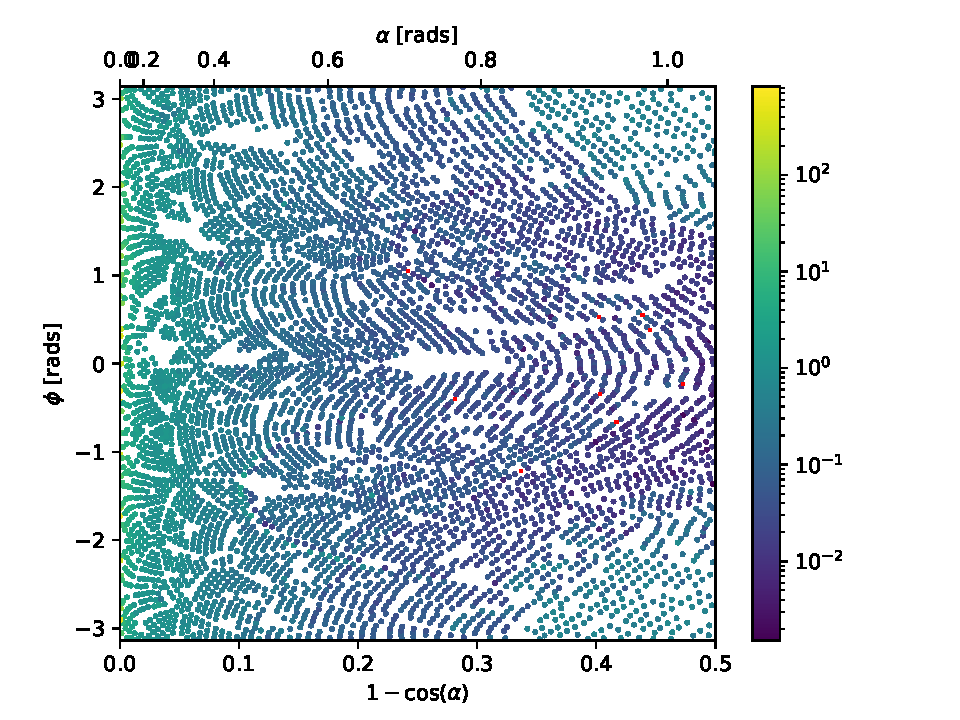
\includegraphics[width=\textwidth]{images/flat_plot_r_FS055_beam_profile_use_f_actual_profile.pdf}
    \caption{Updated beam profile, after combining multiple data sets, for fibre FS055. Once again, the relative intensities ($b_{i}$) for each PMT are given by the color of each point, the position of each plotted in the 2D $(r,\phi)$-space. Red points are PMTs that, even after all relevant subruns have been combined, have no PMT hits.}
    \label{fig:updated_beam_profile}
\end{figure}
Further details can be gathered from the interpolated intensity maps, one of which can be seen in figure~\ref{fig:updated_beam_profile_sampling}. There are two curious stand-out features that can be seen here: firstly, there are multiple distinct parabolic arcs. These correspond to the shadows of the ropes that hold up/down the AV. More precisely, they are the mis-modelling of those shadows --- if the shadows were in the right place in the isotropic MC, then they would correctly cancel out any decreased intensity seen in the data of shadowed PMTs. These shadows could be mis-modelled either because the positions of the ropes in the MC are in the wrong place, or the fibre's emission position is wrong. Note that any mis-modelling of the fibre's nominal emission direction has no impact on this shadowing problem, as changing that direction merely causes a change of basis in the $(r,\phi)$-space. The latter possibility of incorrect fibre positions are more likely, and in fact these arcs in the beam profiles could be used as an effective way to correct for this problem.
\begin{figure}[ht]
    \centering
    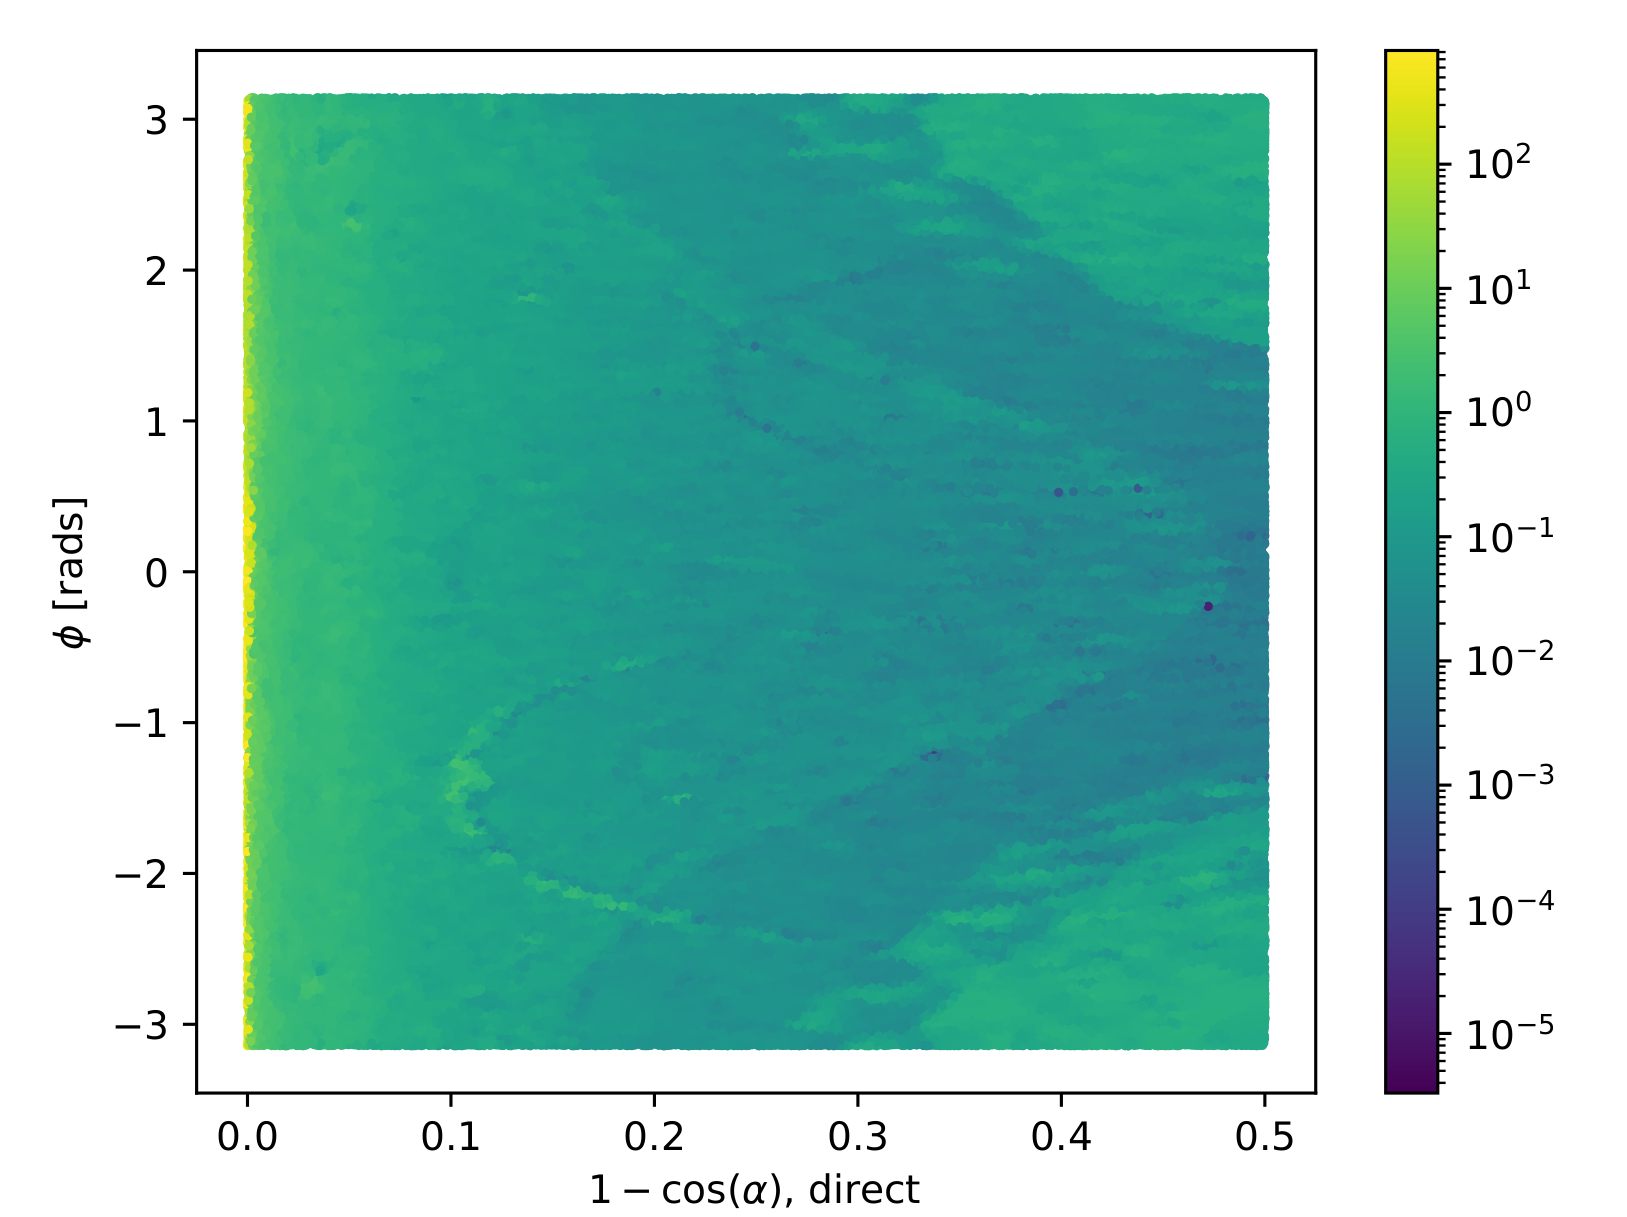
\includegraphics[width=\textwidth]{images/flat_plot_FS055_MC_sampling_new_beam_profile.png}
    \caption{Interpolated intensity map for the new updated beam profile of fibre FS055. The mis-alignment of rope shadows and AV effects, can both be seen.}
    \label{fig:updated_beam_profile_sampling}
\end{figure}
The second distinctive feature of this intensity map is the large band of lower intensity varying between $r\approx0.2-0.5$, followed by larger intensity out at large $r$ values. This feature comes from light reflecting off of the AV surface, or internally-reflecting. The reason for this band's functional dependence on $\phi$ is that this particular fibre, FS055, has a nominal fibre direction $\sim\ang{10}$ from pointing radially-towards the detector's centre. This feature appears in the updated beam profiles of all fibres, but its shape depends in the particular fibre's nominal fibre direction --- for fibres pointing directly towards the detector's center, there is little $\phi$-dependence observed. Like the ropes, this feature must come from some form of mis-modelling of the optics of the AV. A de-facto shadowing of PMTs along lines running from the fibre position running tangent the AV surface, as well as an boosted intensity just beyond this, is to be expected. However, the discontinuities seen in the beam profiles indicate that for whatever reason this effect has been over-emphasised in the simulation.

There is a further phenomenon that can be seen, by comparing beam profile values obtained from a single subrun to the updated combined beam profile. This can be done by calculating the $X_{i}$ values corresponding to the single subrun, relative to the combined data set. For example, looking again at figure~\ref{fig:likelihood_scan}, the single subrun shown has a maximum likelihood estimate of $b_{i}\approx 1.88$. Then, looking at the value of $X_{i}$ for the combined data sets at that $b_{i}$ value, we get a number a little beyond 10. To add a further bit of information, this value is given a further negative sign if the combined data sets have a $b_{i}$ below the equivalent for this single subrun; that is, the combined model underestimates this subrun for that PMT.

This information was plotted for two different subruns from the same fibre, seen in figure~\ref{fig:llr}. One subrun was the same one used by Esther Turner for the original 2D beam profiling, with a wavelength of \SI{495}{\nano\metre}; the latter was at the longer wavelength of \SI{595}{\nano\metre}. For both subruns, most PMTs are seen to have intensities well-modelled by the combined model. However, their appears to be a significant amount of mis-modelling within the beamspot. There also appears to be some systematic shift between data and model at somewhat larger polar angles. Moreover, this mis-modelling seems not to be merely random, but a function of wavelength: at shorter wavelengths the beamspot tends towards being overestimated and then underestimated at larger values of $\alpha$. At longer wavelengths, the beamspot becomes underestimated, with larger angles getting overestimated. This indicates that there appears to be a wavelength-dependence on the beam profiles, contradicting one of the main assumptions which we used to combine the water-phase data in the first place!
\begin{figure}[ht]
    \centering
    \begin{subfigure}{0.98\textwidth}
        \centering
        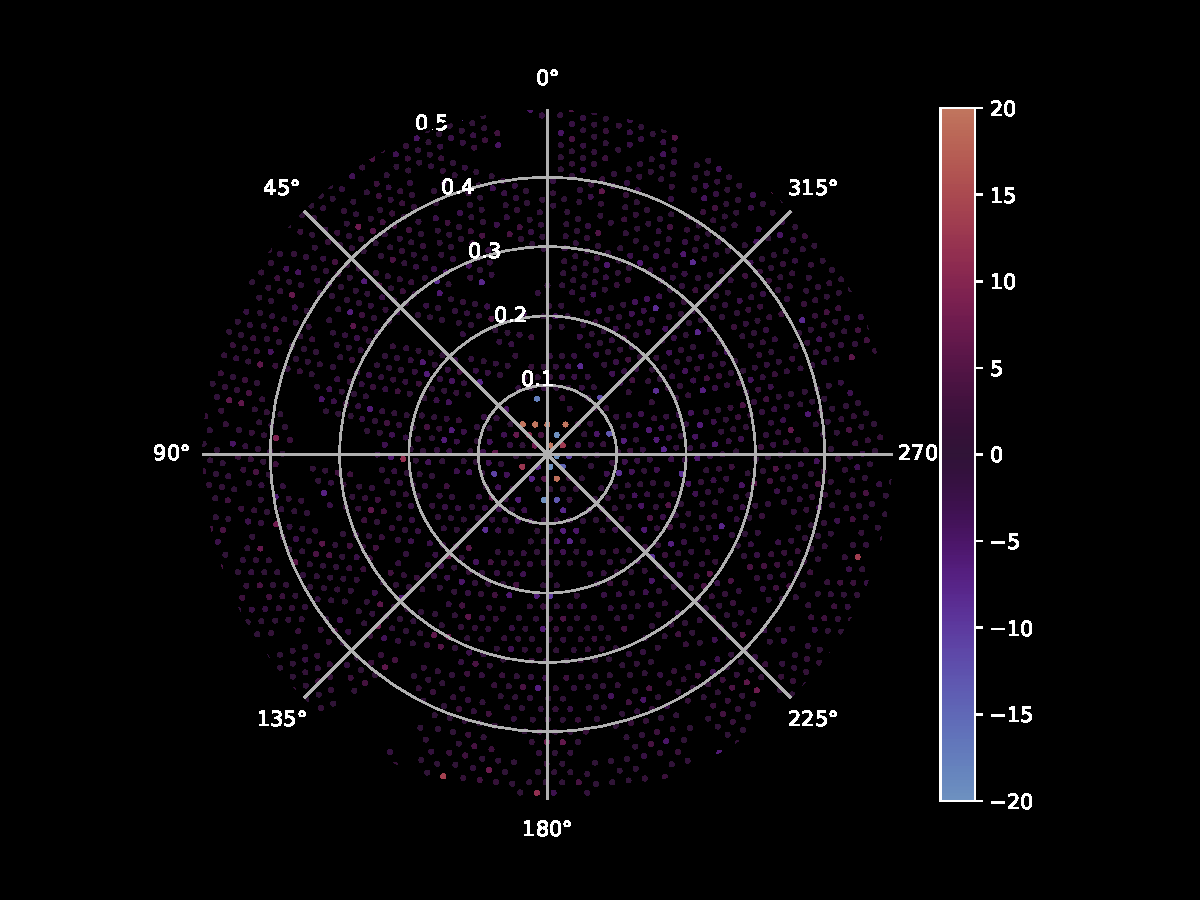
\includegraphics[width=0.8\textwidth]{images/llr_polar_FS055_114018_109_hist_method_use_f_zoomed_data_to_model.pdf}
        \caption{\SI{495}{\nano\metre}}
        \label{fig:llr_495nm}
    \end{subfigure}
    \begin{subfigure}{0.98\textwidth}
        \centering
        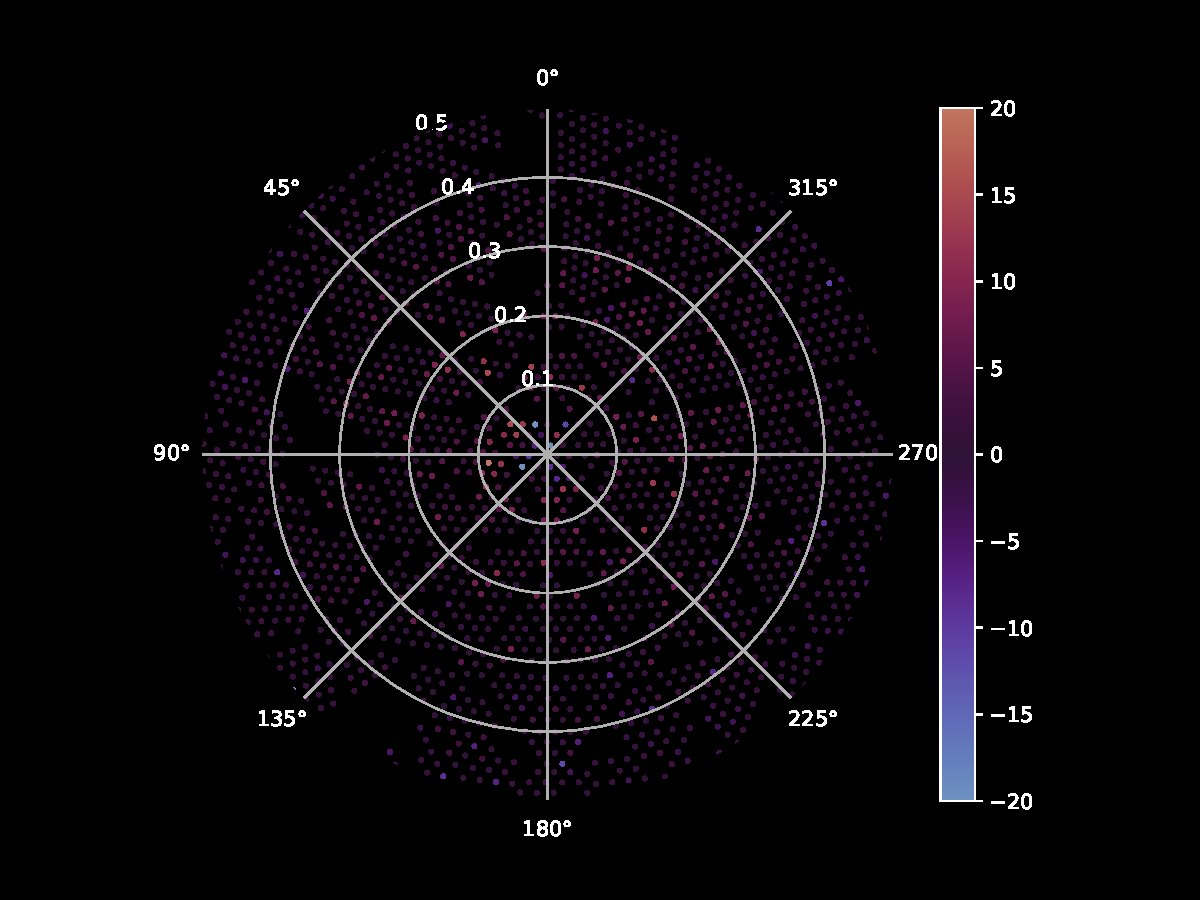
\includegraphics[width=0.8\textwidth]{images/llr_polar_FS055_114034_39_hist_method_use_f_zoomed_data_to_model.pdf}
        \caption{\SI{595}{\nano\metre}}
        \label{fig:llr_595nm}
    \end{subfigure}
    \caption{$X_{i}$ values from subruns at two different wavelengths, both compared to the combined beam profile model for fibre FS055. A negative sign, and hence bluer colours, indicate that the combined model underestimates the observed intensity for that particular subrun. Values with a magnitude beyond 20 are shown capped at this maximal value for the purposes of this plot. These PMTs are plotted in the polar fibre coordinates $(\alpha,\phi)$.}
    \label{fig:llr}
\end{figure}
All three of these features --- rope shadows, AV reflections, and wavelength dependence --- add systematic uncertainty to the beam profiles, beyond the statistical uncertainty as measured by the width of the likelihood distribution. Certainly if one wanted to further improve the uncertainties in the beam profiles, tackling these challenges would be key.